\chapter{Introduction}

% Trends of the electronic field is size reduction
La miniaturization des circuits électroniques se poursuit malgré des barrières technologiques de plus en plus élevées.
La diminution de taille des circuits intégrés permet une réduction des coûts grâce à l'augmentation des volumes de production.
La réduction de poids des modules électroniques pour l'automobile ou l'aéronautique permet des réductions de carburant, de coût, et moins d'impact sur l'environnement.
A taille constante, des circuit intégrés plus denses peuvent embarquer plus de fonctionnalités et ont des performances plus élevées.

% How is size reduced
La réduction de taille des circuits intégrés est possible en utilisant des technologies silicium plus fines.
Une technologie silicium définie les dimensions et les formes d'un ensemble de briques de conception électronique, formant une librairie de composants, ainsi que tous les procédés nécessaires à la fabrication du circuit intégré.
La plupart du temps, ces librairies de composant sont constituées de différents types de transistors, diode, résistances et capacitances.
La taille d'une technologie est définie par la plus petite dimension possible pour une grille de transistor, aussi appellée \textlambda.
La valeur de \textlambda est essentielle et conditionne fortement la taille du circuit final, sa consommation et ses performances.
Jusqu'à présent, la loi de Moore a prédit avec succès que \textlambda serait réduit d'un facteur deux tous les dix-huit mois.
Le domaine automobile se conforme à cette tendance, en utilisant récemment des noeuds technologiques à 16nm (Fig. \ref{fig:nxp-techno-increase}) \cite{evolution_technologies} normalement utilisés dans des applications moins sévères.

\begin{figure}[!h]
  \centering
  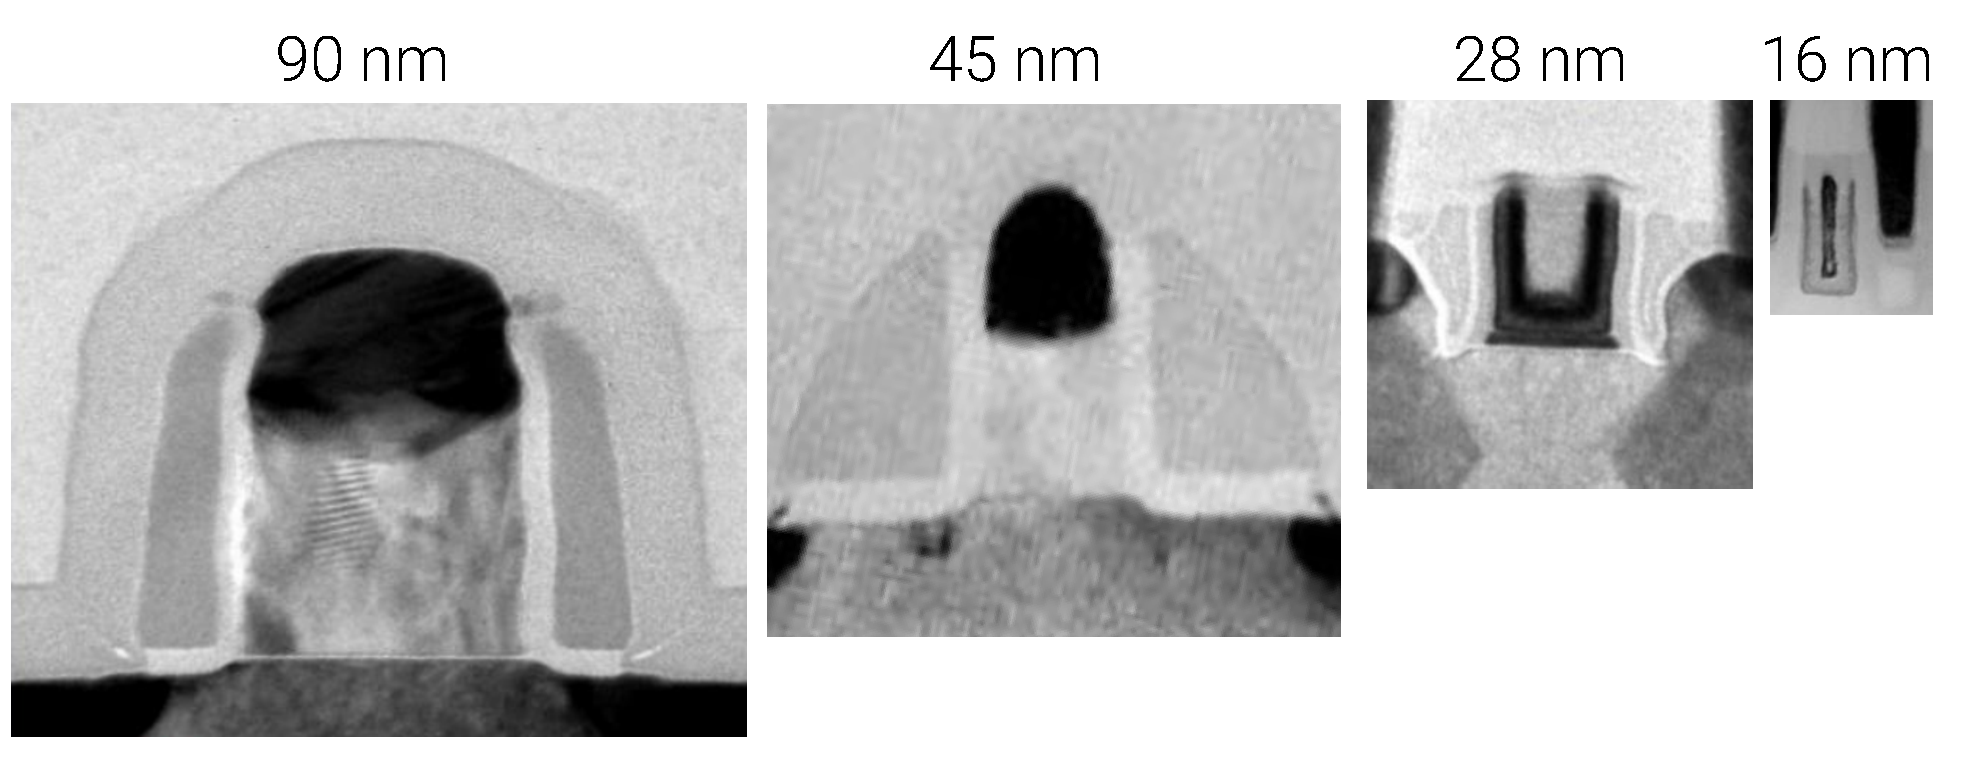
\includegraphics[width=\textwidth]{src/1/figures/technology_evolution.pdf}
  \caption{Recent evolution of NXP's automotive technology nodes \cite{evolution_technologies}}
  \label{fig:nxp-techno-increase}
\end{figure}

% Side effects of size reduction
Cette réduction de taille s'accompagne d'une augmentation de la fragilité et de la sensibilité des circuits intégrés.
Les seuils de tolérances en tension et courant deviennent plus petits, au delà desquels les circuits sont détruits.
La surface de silicium nécessaire à la protection des coeurs de circuits occupe une plus large part de l'aire totale d'un produit  \cite{evolution_technologies}, et donc du coût.

% Another trend in automotive - more electronic functions
De nos jours, de nouvelles fonctionnalités majeures sont aussi en dévelopement dans le domaine automobile.
En particulier, les véhicules autonomes ou l'aide à la conduite font leur apparition sur les routes.
Ces fonctionnalités font en permanence des décisions et prennent des actions critiques sur le véhicule, comme tourner le volant ou enclencher le freinage.
Elles sont implémentées afin d'augmenter la sécurité des usagers d'un véhicule, ce qui résulte en des responsabilités et des contraintes accrues sur les modules électroniques.
La sûreté de fonctionnement des ces modules est donc vitale pour ce type d'application.

% Another trend is reduced power consumptions
L'augmentation de la quantité d'électronique dans un véhicule s'accompagne aussi d'une forte hausse de la consommation électrique.
Au niveau circuit-intégré, les tensions d'alimentations sont réduites très bas, avec communément des seuils d'alimentions de 1V.
Les marges de bruit des cellules digitales sont réduites d'autant, rendant les circuits bien plus sensibles aux perturbations électriques.

% Harsh environment in the automotive field
Par ailleurs, l'environnement automobile est très sévère pour les composants électroniques.
Un moteur en fonctionnement génère de la chaleur et des vibrations.
Durant toute sa vie, un véhicule est exposé à de larges cycles thermiques.
Les contacts électriques, les soudures et les connections vieillissent plus rapidement à cause de cela.
De plus, les systèmes électroniques sont exposés à une large plage de stress électriques.
Quand le moteur est allumé, la tension de batterie chute fortement à cause de l'appel de courant créé par le démarreur.
Cette variation très brutale peut affecter ou endommager les modules.
Il existe également une autre famille de perturbations électriques appellée décharges électrostatiques, et produite par l'environnement du véhicule.

% What is an ESD
Une décharge électrostatique est un transfert de charge soudain entre deux objets de différente charge.
C'est le résultat d'une accumulation de potentiel électrostatique.
La décharge se produit lorsque la différence de potentiel est suffisamment large.
L'amplitude de tels événements peut atteindre couramment plusieurs milliers de volts et des dizaines d'ampères.
Le fabricant de véhicules Renault estimes que les composants électroniques automobiles sont exposés 10000 fois à des décharges pendant leur vie \cite{Renault-esd}.

% Architecture systemes automobiles
L'architecture des systèmes électriques dans un véhicule est également très complexe et rude pour les modules électroniques.
Une voiture est consistutées d'une multitude de modules électroniques interconnectés par des câbles.
C'est un vrai challenge pour garantir la robustesse de cet ensemble contre des perturbations électriques.
La seule connection d'une voiture à une vrai référence électrique se fait par les pneus, ce qui équivaut globalement à une très mauvaise connection à la terre.
Néanmoins, les modules électroniques ont besoin d'une bonne référence pour communiquer entre eux et fonctionner correctement.
Ceci est assuré par la carcasse métallique du véhicule.
En statique et à basse fréquence, cette référence est très bonne car très peu résistive.
Les décharges électrostatiques sont au contraire des évènements avec la majorité du spectre à très haute fréquence, jusqu'à 1 GHz environ.
Dans cette gamme de fréquence, la carcasse métallique ne se comporte plus comme une bonne référence et les cables deviennent largement inductifs.
Ces phénomènes peuvent donc fortement perturber les systèmes électroniques.
De plus, les cables peuvent rayonner et les propagations peuvent se propager par couplage.
Globalement, l'architecture d'un véhicule est complex et sensible par nature aux perturbations.

\begin{figure}[!h]
  \centering
  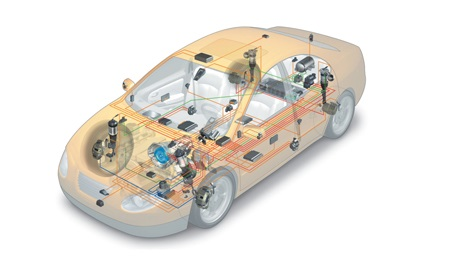
\includegraphics[width=0.6\textwidth]{src/1/figures/systemintegration_01_uv-data.jpg}
  \caption{Architecture of electronic systems in a vehicle \cite{car-architecture}}
  \label{fig:car-architecture}
\end{figure}

% Fiabilite vis a vis des ESD
En résumé, la quantité de composants électroniques est en augmentation et en parallele ils deviennent de plus en plus sensibles.
De plus, ils doivent opérer dans une environnement électrique sévère, avec de multiples sources de perturbation.
Ces perturbations peuvent créer des défaillances.
Dans le domaine des décharges électrostatiques, il y a deux types de défaillances à considérer.
La casse matérielle est le résultat de la destruction permanente d'un composant.
Les circuits intégrés sont particulièrement vulnérables \cite{impactESDsemiconductors} et nécessitent des mesures de protection.
Récemment, un deuxième type de défaillance commence à être étudié.
Les défaillances fonctionnelles sont une perturbation d'une fonction électrique du circuit intégré à la suite d'une décharge.
Plusieurs niveaux de sévérité existent.
La perturbation du système d'airbag est par exemple bien plus critique celle du système de tableau de bord.

\begin{figure}[!h]
  \centering
  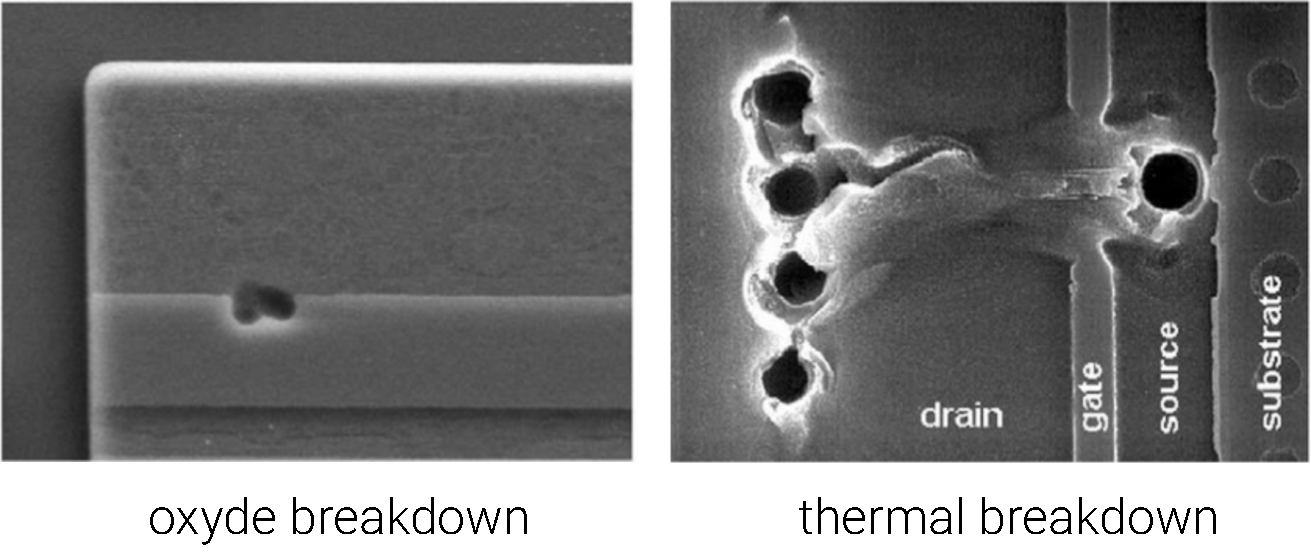
\includegraphics[width=0.4\textwidth]{src/1/figures/esd_failures.jpg}
  \caption{Different kinds of ESD-induced failures}
  \label{fig:esd-failures}
\end{figure}

% Comment predire ces defaillances fonctionnelles
Des travaux sur ce sujet ont été publiés par F. Caignet et N. Lacrampe en 2007 \cite{}.
Egalement, de nombreuses recherches sur les défaillances au niveau système ont été publiées pendant les symposia EOS/ESD 2012 \cite{} et 2013 \cite{}.
De plus, le standard IEC 62433-6 encore en phase d'élaboration cherche à formaliser des méthodes de base pour l'analyse et la prédiction de faiblesses fonctionnelles.
Globalement, les recherches dans ce domaine restent focalisées au niveau système.
Dans ce document, la recherche et l'analyse de faiblesses fonctionnelles a lieu plus bas dans la hiérarchie, au niveau circuit-intégré.

% Presentation des chapitres
%
Le chapitre \ref{chap:1} fournit en détail les notions essentielles à la compréhension de la problématique.
Il explique comment les décharges électrostatiques apparaissent et comment elles sont reproduites en laboratoire.
Ensuite, une revue de l'état de l'art est présentée sur l'analyse des pertes de fonctionnalités dues à des décharges.

%
La chapitre \ref{chap:2} présente un méthode de modélisation pour simuler la propagation de décharges électrostatiques jusqu'au composant.
C'est une part important du problème que d'identifier quelle fraction d'une décharge atteint réellement un circuit intégré.
Une librairie de modèles est construite, ensuite assemblés ensemble pour reproduire le système à simuler.
Un générateur de stress utilisé dans le laboratoire de test à NXP est modélisé pour illustrer la méthode.
Un nouveau générateur de stress, appellé TLP-HMM est ensuite proposé, reproduisant une forme d'onde standardizée mais avec des avantages importants sur les générateurs actuels.
Ce générateur est particulièrement intéressant pour effectuer des tests de décharge sur circuits intégrés.

%
Un cas de défaillance fonctionnelle est ensuite présenté dans le chapitre \ref{chap:3}.
Tout d'abord, des mesures sont effectuées de manière externe sur le circuit intégré sous test.
La signature de la défaillance est expliquée.
Ensuite, un circuit intégré de test est développé et fabriqué sur silicium.
Il contient des structures spéciales pour mesurer les pertubations directement depuis le silicium.

%
Ces travaux ont aussi été orientés vers la recherche de nouvelles méthodes de simulation.
L'objectif est de détecter plus facilement et rapidement des défaillances fonctionnelles, en utilisant les outils existants de simulation.
Trois méthodes différentes sont présentées dans le chapitre \ref{chap:4}.
Elles ont chacune des applications différentes, mais peuvent s'avérer complémentaires pour concevoir des circuits robustes.

%
Enfin, la conclusion résume les travaux effectués et présente des axes de recherche futurs.
